\documentclass{rapport}
\usepackage[utf8]{inputenc}
\usepackage[T1]{fontenc} 
\usepackage{pifont} % Pour les symboles appelés par la macro \ding
\usepackage{url} % Comme son nom l'indique, pour les url...
\usepackage{amssymb}
\usetikzlibrary{positioning} % Bibliothèque tikz pour positionner des nœuds relativement à d'autres

\usepackage[colorlinks, citecolor=red!60!green, linkcolor=blue!60!green, urlcolor=magenta]{hyperref} % Pour que les liens soient cliquables. Les options permettent de mettre les liens en couleur.

\usepackage{mathrsfs}
\usepackage{pgfplots}
    
\usepackage{algorithm}
\usepackage{algo}
\usepackage{colorationSyntaxique}


% Pour un rapport en français 
\usepackage[french]{babel} % Commenter pour un rapport en anglais
\renewcommand\bibsection{\section*{Bibliographie}} % Commenter pour un rapport en anglais

% \englishTitlePage % Décommenter pour une page de titre en anglais


\pagestyle{fancy}
\renewcommand{\sectionmark}[1]{\markboth{\thesection.\ #1}{}}
\fancyfoot{}

\fancyhead[LE]{\textsl{\leftmark}}
\fancyhead[RE, LO]{\textbf{\thepage}}
\fancyhead[RO]{\textsl{\rightmark}}

\def\Latex{\LaTeX\xspace}
\def\etc{\textit{etc.}\xspace}



\title{Extraction automatique de ContextMaps dans des architectures micro-services}
\author{Thomas FARINEAU, Léo KITABDJIAN, Mohamed MAHJOUB}
\supervisor{Philippe COLLET}
\date{Second semestre de l'année 2023-2024}

 \universityname{Université Côte d'Azur} % Nom de l'université.
 \type{PER} % Type de document
 \formation{SI5 AL / M2} % Nom de la formation


\begin{document}
  \maketitle
    \begin{abstract}
L'évolution rapide des architectures logicielles vers des architectures en micro-services, a engendré un besoin croissant de méthodologies et d'outils facilitant la compréhension, la maintenance et l'évolution de ces systèmes complexes. L'intégration des principes de Domain-Driven Design (DDD)  s'est révélée bénéfique pour la conception de micro-services en favorisant une représentation métier claire et des frontières de contexte explicites \cite{articleDDD}.

Cependant, la rétro-ingénierie, de systèmes existants adoptant ces architectures représente souvent un défi majeur. La complexité intrinsèque des micro-services, avec leurs multiples interdépendances et leur distribution, nécessite des outils spécialisés pour extraire et interpréter efficacement les concepts DDD intégrés. C'est dans ce contexte qu'émerge la problématique à laquelle cette recherche souhaite répondre : la création d'un outil dédié à l'analyse du DDD dans les architectures en micro-services, simplifiant ainsi le processus de rétro-ingénierie.

L'objectif principal de ce projet est de développer un outil permettant d'analyser les architectures en micro-services à la lumière des principes DDD \cite{evans2003,vernon2013}. L'outil visera à extraire automatiquement les concepts métier, à identifier les agrégats et à faciliter la compréhension des interactions entre les micro-services. La rétro-ingénierie des systèmes existants sera grandement simplifiée, permettant aux développeurs, architectes et décideurs informatiques de prendre des décisions éclairées concernant l'évolution et la maintenance des systèmes existants.\\\\
(AJOUTER PLAN ICI)\\\\

L'outil principal sur lequel nous pouvons nous baser est Context Mapper \cite{contextmapper,contextMapperGitHub}. Context Mapper se distingue par ses fonctionnalités spécifiques qui simplifient la modélisation de domaines complexes. La délimitation des contextes, une caractéristique phare de l'outil, offre aux développeurs la possibilité de séparer clairement les concepts spécifiques à chaque partie du système \cite{mdslMedium2021}. Cette approche structurée facilite la compréhension des interactions au sein du domaine, favorisant ainsi une modélisation plus précise et pertinente.

La modélisation d'Entités, Objets de Valeur et Agrégats constitue un autre aspect essentiel de Context Mapper, s'alignant parfaitement avec les principes du Domain-Driven Design (DDD). En permettant aux développeurs de représenter ces composants clés de manière structurée, l'outil encourage une conception logicielle centrée sur le domaine, assurant ainsi une adéquation étroite avec les besoins métier.

    \begin{figure}[ht]
        \centering
        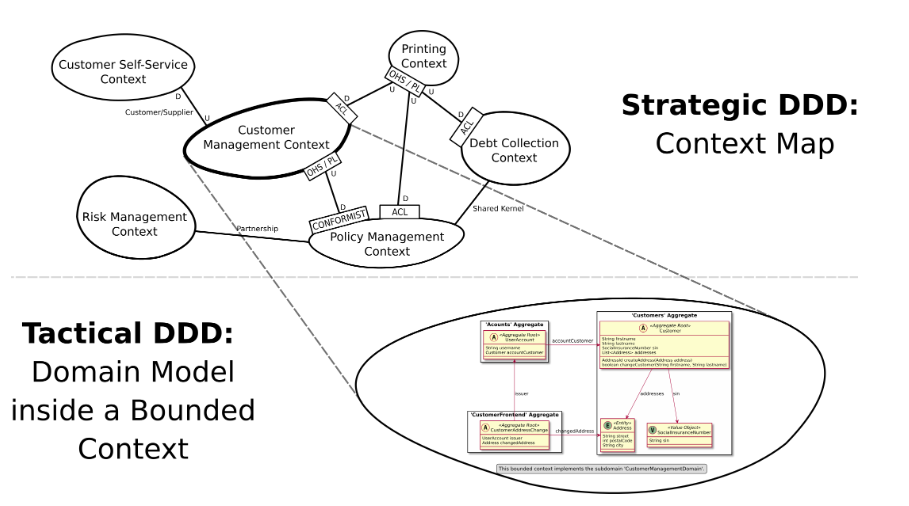
\includegraphics[width=0.5\linewidth]{img/ExempleMapper.png}
        \caption{Exemple d'un mapping donné par Context Mapper \cite{insuranceExampleGitHub}}
    \end{figure}


Dans le cadre de notre projet, nous avons entrepris une analyse approfondie en vue d'améliorer Context Mapper Discovery \cite{contextMapperDiscoveryDocs,contextMapperDiscoveryGitHub}, un outil déjà développé au sein de Context Mapper. Cependant, cette exploration a mis en lumière plusieurs défis inhérents à Context Mapper Discovery, parmi lesquels l'incompatibilité avec la version Spring 3.0, limitant ainsi la flexibilité des technologies utilisées. De plus, la fonctionnalité de l'outil s'est avérée trop spécifique, orientée principalement vers le projet d'exemple fourni, ne garantissant pas une adaptabilité universelle. Des erreurs liées à des spécificités non documentées, telles que des conventions de nommage imposées sans explication, ont également été identifiées.

Un autre problème a émergé avec la limitation de Context Mapper Discovery à Java Spring, restreignant ainsi son champ d'application. Par ailleurs, le manque de détails sur les agrégats exposés entre les contextes a été souligné, car le découvreur ne fournissait qu'une liste générique au lieu de comprendre de manière approfondie les données effectivement échangées.

Face à ces challenges, nous avons dû imaginer une solution pour enrichir Context Mapper Discovery. Nous avons tout d'abord considéré l'idée de prendre les problèmes un à un et de les réparer individuellement, cependant cette solution a vite été abandonnée après réflexion car, à cause d'un manque de documentation complète du fonctionnement de Context Mapper Discovery, il est difficile d'isoler tous les problèmes. Nous avons donc imaginé une solution alternative, il s'agirait de reconstruire Context Mapper Discovery, cette solution a pour avantage de garder l'outil Context Mapper tout en créant Discovery pour répondre à nos besoins, cependant cette solution a aussi été abandonnée car elle aurait requis un fort coût en temps de travail et elle ne nous aurait pas permis de régler les problèmes de limitations de langages au Java Spring.

Nous avons donc choisi alternative final de créer notre propre outil (semi-)autonaume de context mapping et service discovery,nous avons examiné plusieurs options pour l'analyse rétrospective des architectures en micro-services. Notre solution étant autonome, nous avons donc la possibilité de choisir les technologies et méthodes que nous voulons utiliser, tout d'abord, nous avons envisagé de nous orienter vers l'analyse de fichiers OpenAPI/Swagger \cite{openapi_spec}. Un autre avantage du développement de notre solution autonome est la liberté du choix du langage de programmation. Nous avons considéré Java et Node.js, mais avons finalement choisi Node.js car celui-ci offre une plus grande liberté dans le choix des bibliothèques.

Nous avons priorisé les bibliothèques les plus populaires pour notre projet. Parmi de nombreuses options disponibles, nous avons écarté celles peu utilisées ou manquant de documentation exhaustive. Notre critère de sélection s'est basé sur le nombre d'étoiles sur GitHub et le volume de téléchargements hebdomadaires, ce qui nous a amenés à choisir entre ReDoc et Swagger Parser.

ReDoc \cite{redoc} ,est attrayant car il supporte OpenAPI 3.1, offrant ainsi une compatibilité avec les spécifications les plus récentes. Cependant, sa fonctionnalité principale ne cible pas du tout notre besoin et fait de ReDoc une librairie trop large/lourde pour ce que l’on souhaite (valider un fichier OpenApi et le transformer en objet parsable).

D'autre part, Swagger Parser \cite{swagger_parser}, bien qu'il ne prenne en charge que jusqu'à OpenAPI 3.0, est adapté pour nos besoins actuels qu’il cible parfaitement sans proposer de fonctionnalités superflues. Il bénéficie d'une large base d'utilisateurs, comme en témoignent ses nombreux téléchargements, et d'une documentation complète et accessible. 
Ces facteurs, combinés à sa simplicité relative par rapport à ReDoc, rendent Swagger Parser particulièrement adapté à nos objectifs. Enfin, la version OpenAPI 3.1 ne rajoute que très peu de fonctionnalités et aucune d’entre elles n’affecte notre application ou son fonctionnement.

Concernant la modélisation des données, la nature des fichiers OpenAPI/Swagger, qui décrivent un service individuel plutôt qu'un ensemble de services et de leurs relations, a suscité une réflexion approfondie. Pour établir les relations entre ces services, nous envisageons d'adopter la méthode de Context Mapper Discovery en utilisant un fichier Docker Compose \cite{docker_compose} ,pour définir les communications entre les services. À l'intérieur des fichiers Swagger, les routes du service et, de manière cruciale, les schémas des données transitant sur ces routes, représentent une source d'informations précieuses. Nous projetons d'utiliser ces données pour construire la section relative aux données des contextes limités, voire des agrégats exposés d'un service à un autre, avec une précision accrue par rapport à Context Mapper Discovery. Cette approche implique une analyse des schémas similaires entre les services qui communiquent, s'appuyant sur le fichier Docker Compose.

Nous avons donc imaginé l'architecture suivante pour notre Solution


    
    \begin{figure}[ht]
        \centering
        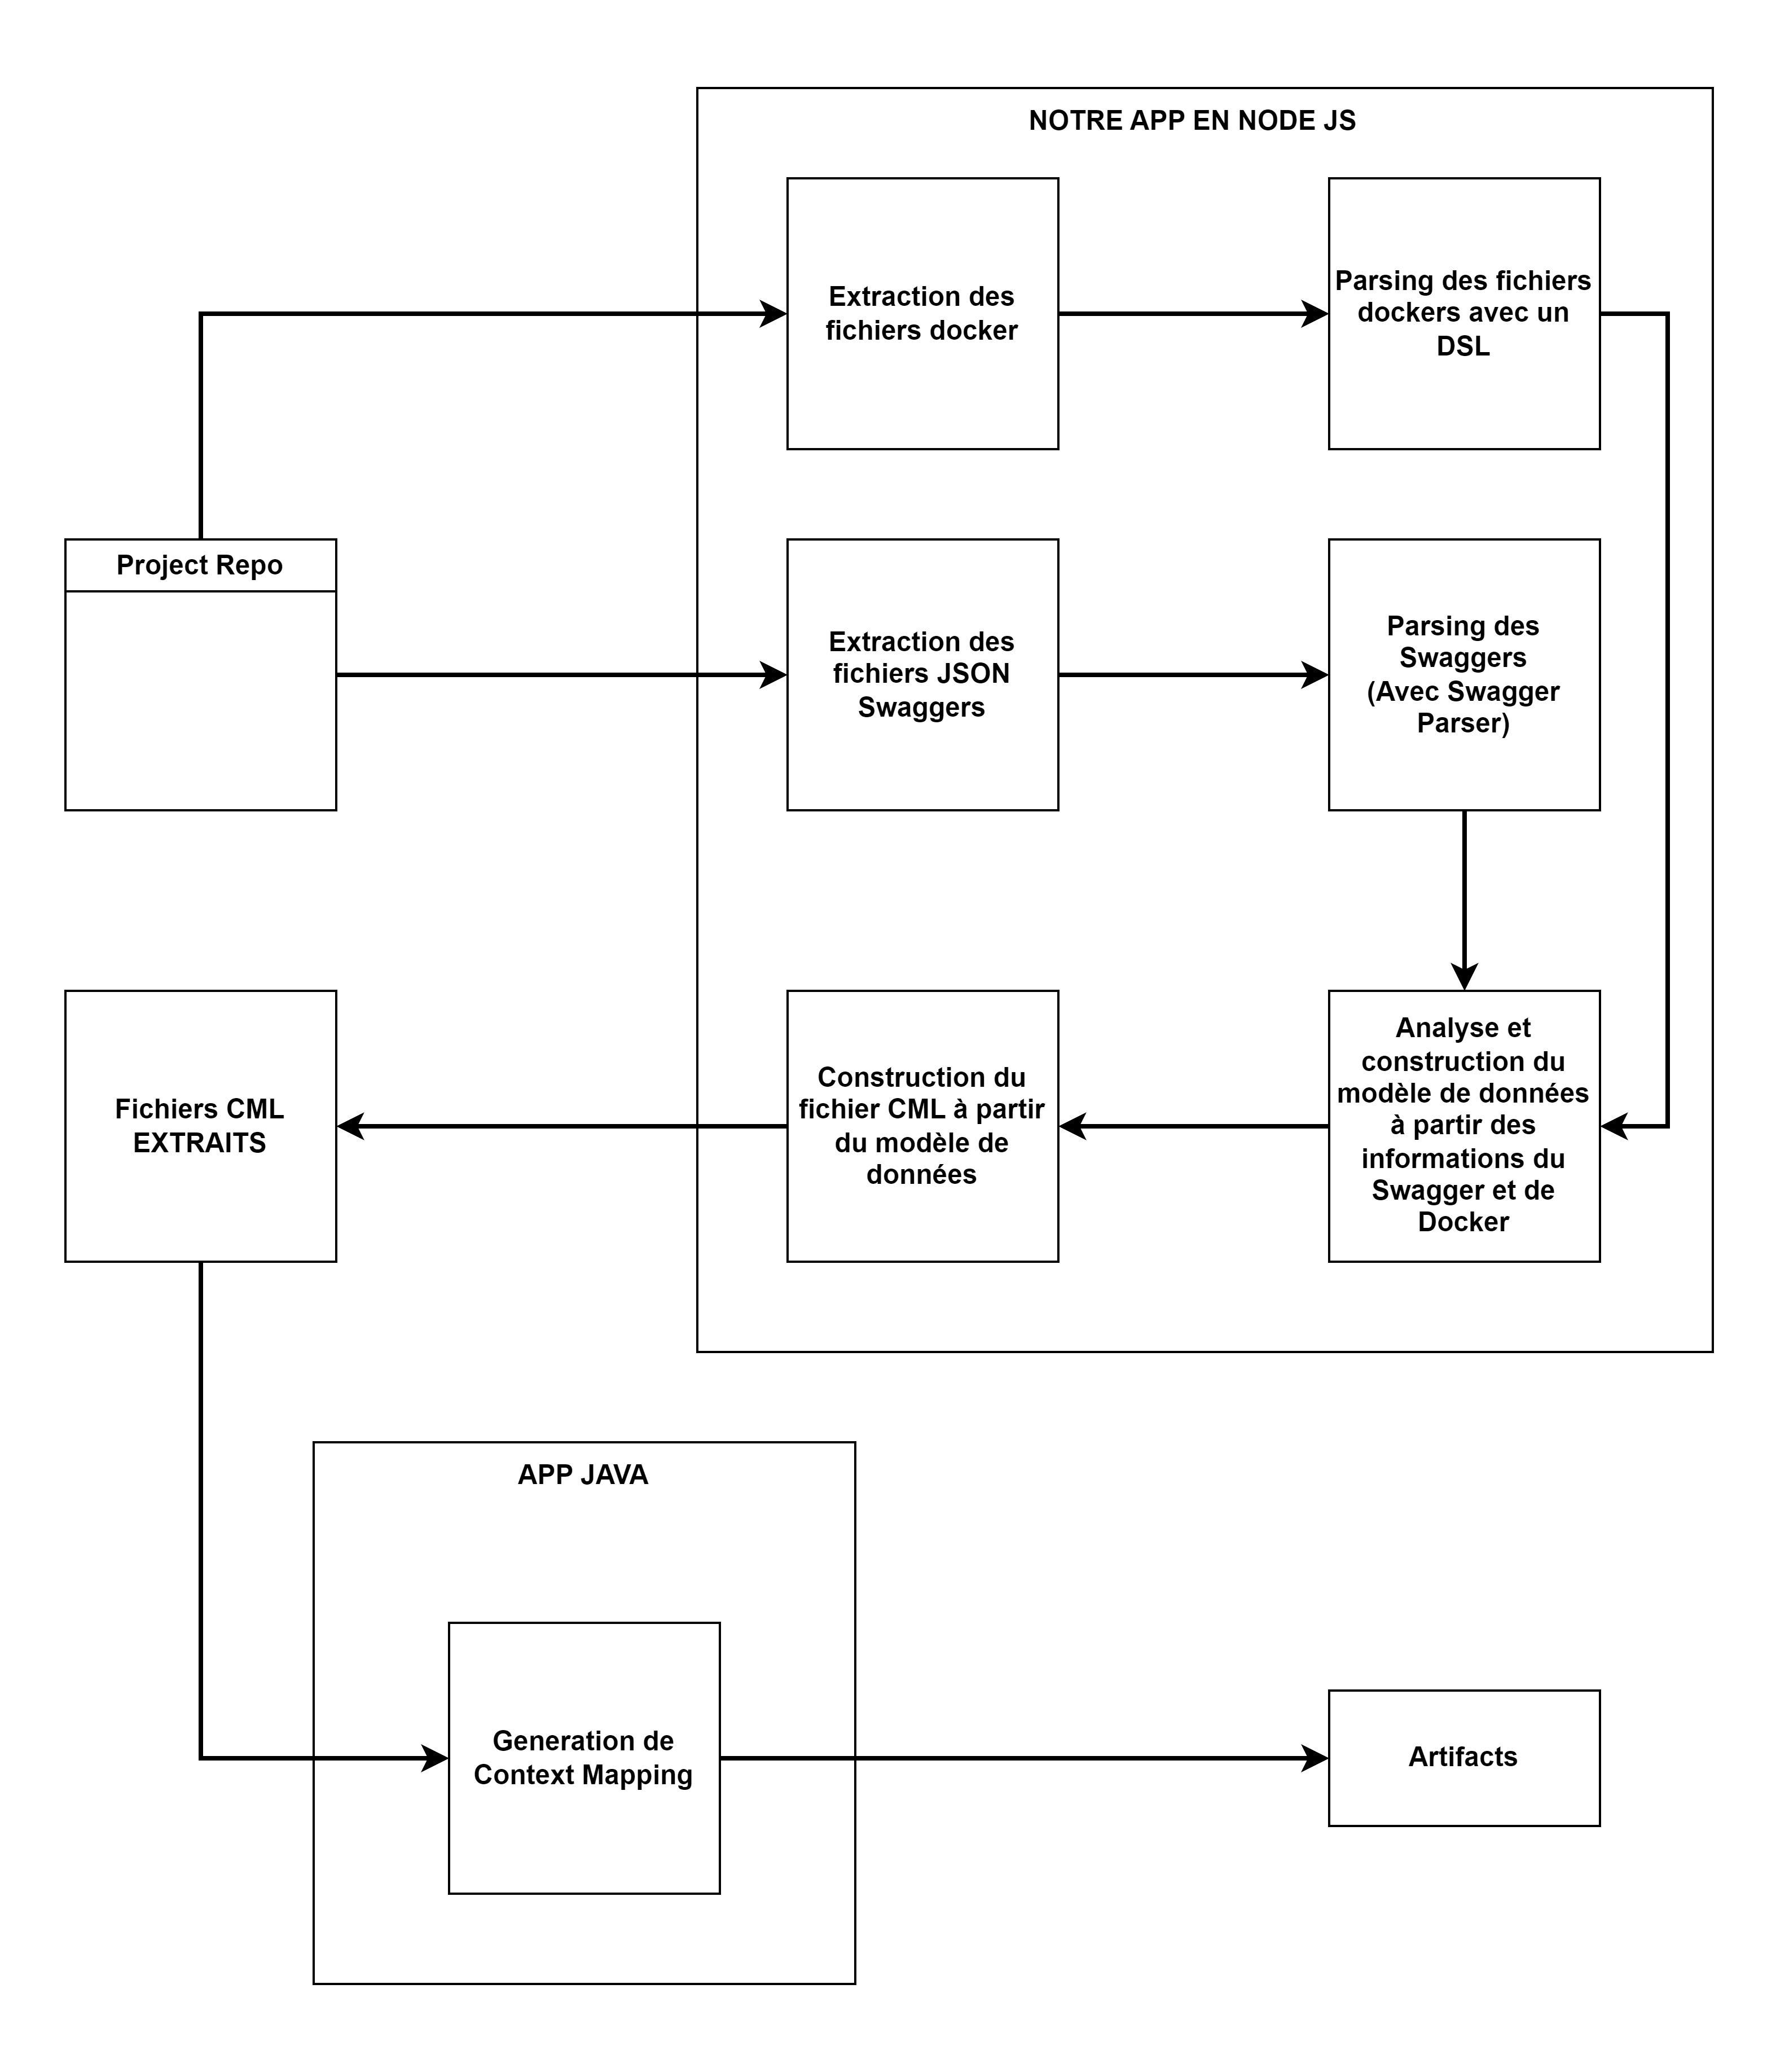
\includegraphics[height=14cm]{img/ContextMapper.png}
        \caption{Architecture prévue pour notre solution}
    \end{figure}




    \end{abstract}

    \clearpage
    \tableofcontents

    \clearpage
    \bibliographystyle{plain}
    \bibliography{biblio}
\end{document}
